\documentclass[tikz, margin=0.1cm]{standalone}

\usepackage{stix2}
\usepackage{booktabs}

\begin{document}
\footnotesize
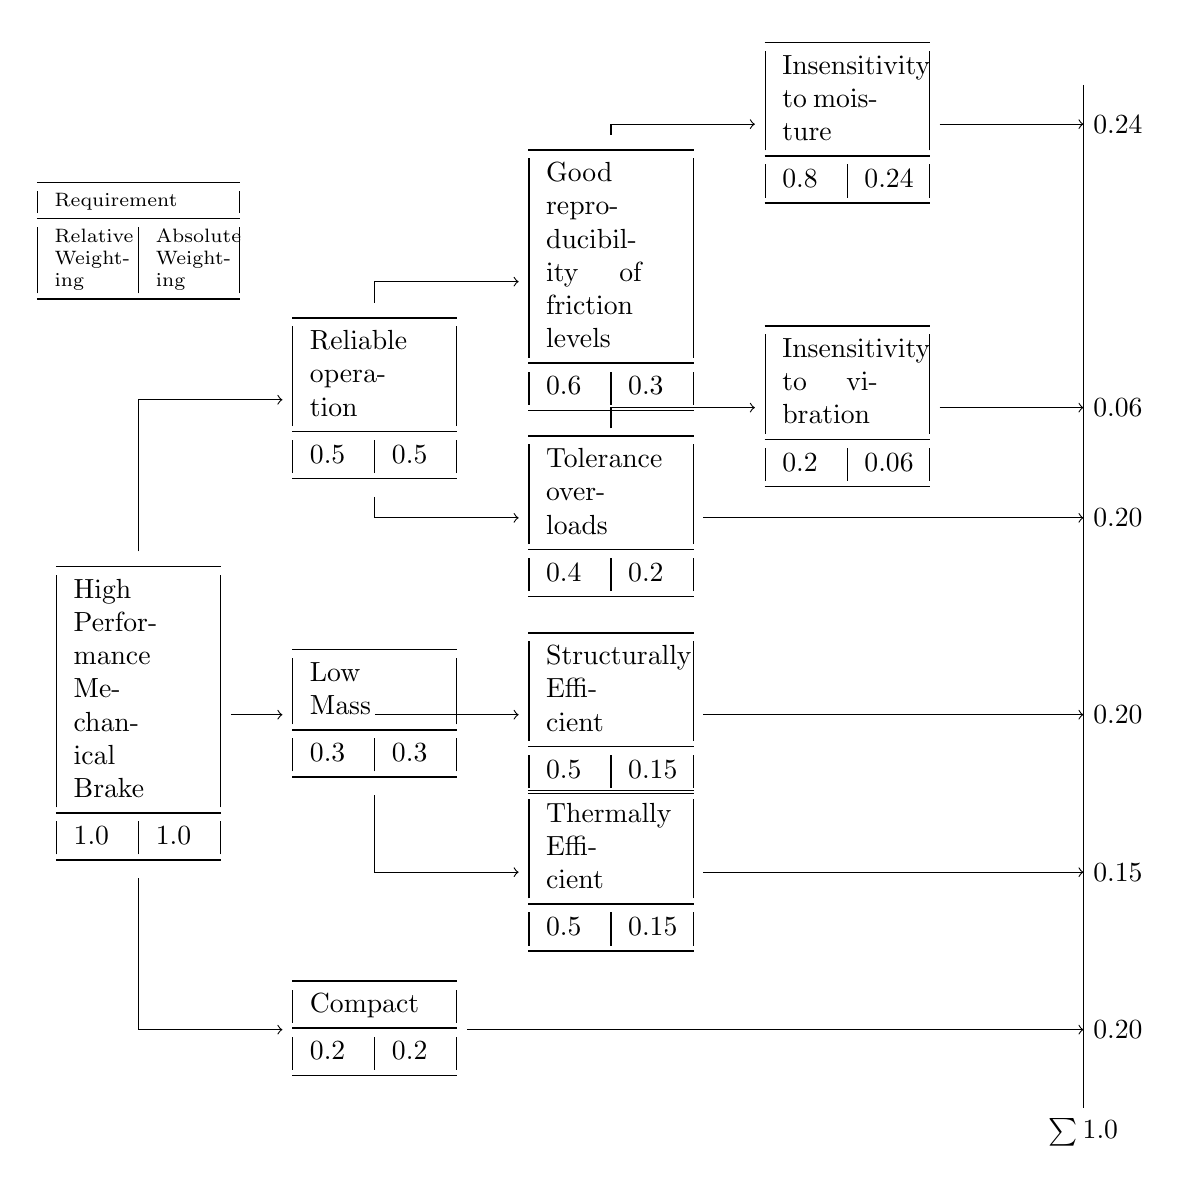
\begin{tikzpicture}

  \node[] (Legend) at (0,6) {
    \scriptsize
    \begin{tabular}{|p{0.07\textwidth}|p{0.07\textwidth}|}
      \midrule
      \multicolumn{2}{|p{0.1\textwidth}|}{Requirement} \\
      \midrule
      Relative Weighting & Absolute Weighting \\
      \midrule
    \end{tabular}
  };

  \node[] (A) at (0,0) {
    \begin{tabular}{|p{0.05\textwidth}|p{0.05\textwidth}|}
      \midrule
      \multicolumn{2}{|p{0.1\textwidth}|}{High Performance Mechanical Brake} \\
      \midrule
      1.0 & 1.0 \\
      \midrule
    \end{tabular}
  };

  \node[] (B) at (3,4) {
    \begin{tabular}{|p{0.05\textwidth}|p{0.05\textwidth}|}
      \midrule
      \multicolumn{2}{|p{0.1\textwidth}|}{Reliable operation} \\
      \midrule
      0.5 & 0.5 \\
      \midrule
    \end{tabular}
  };

  \node[] (C) at (3,0) {
    \begin{tabular}{|p{0.05\textwidth}|p{0.05\textwidth}|}
      \midrule
      \multicolumn{2}{|p{0.1\textwidth}|}{Low Mass} \\
      \midrule
      0.3 & 0.3 \\
      \midrule
    \end{tabular}
  };

  \node[] (D) at (3,-4) {
    \begin{tabular}{|p{0.05\textwidth}|p{0.05\textwidth}|}
      \midrule
      \multicolumn{2}{|p{0.1\textwidth}|}{Compact} \\
      \midrule
      0.2 & 0.2 \\
      \midrule
    \end{tabular}
  };

  \node[] (E) at (6,5.5) {
    \begin{tabular}{|p{0.05\textwidth}|p{0.05\textwidth}|}
      \midrule
      \multicolumn{2}{|p{0.1\textwidth}|}{Good reproducibility of friction levels} \\
      \midrule
      0.6 & 0.3 \\
      \midrule
    \end{tabular}
  };

  \node[] (F) at (6,2.5) {
    \begin{tabular}{|p{0.05\textwidth}|p{0.05\textwidth}|}
      \midrule
      \multicolumn{2}{|p{0.1\textwidth}|}{Tolerance overloads} \\
      \midrule
      0.4 & 0.2 \\
      \midrule
    \end{tabular}
  };

  \node[] (G) at (6,0) {
    \begin{tabular}{|p{0.05\textwidth}|p{0.05\textwidth}|}
      \midrule
      \multicolumn{2}{|p{0.1\textwidth}|}{Structurally Efficient} \\
      \midrule
      0.5 & 0.15 \\
      \midrule
    \end{tabular}
  };

  \node[] (H) at (6,-2.0) {
    \begin{tabular}{|p{0.05\textwidth}|p{0.05\textwidth}|}
      \midrule
      \multicolumn{2}{|p{0.1\textwidth}|}{Thermally Efficient} \\
      \midrule
      0.5 & 0.15 \\
      \midrule
    \end{tabular}
  };

  \node[] (I) at (9,7.5) {
    \begin{tabular}{|p{0.05\textwidth}|p{0.05\textwidth}|}
      \midrule
      \multicolumn{2}{|p{0.1\textwidth}|}{Insensitivity to moisture} \\
      \midrule
      0.8 & 0.24 \\
      \midrule
    \end{tabular}
  };

  \node[] (J) at (9,3.9) {
    \begin{tabular}{|p{0.05\textwidth}|p{0.05\textwidth}|}
      \midrule
      \multicolumn{2}{|p{0.1\textwidth}|}{Insensitivity to vibration} \\
      \midrule
      0.2 & 0.06 \\
      \midrule
    \end{tabular}
  };

  \draw[] (12,8) -- (12,-5) node[pos=1.0, anchor=north] {$\sum 1.0$};
  \draw[->] (A) |- (B);
  \draw[->] (A) -- (C);
  \draw[->] (A) |- (D);

  \draw[->] (B) |- (E);
  \draw[->] (B) |- (F);

  \draw[->] (C) |- (G);
  \draw[->] (C) |- (H);

  \draw[->] (E) |- (I);
  \draw[->] (E) |- (J);

  \draw[->] (D) -- (12,-4) node[pos=1.0, anchor=west] {0.20};
  \draw[->] (I) -- (12,7.5) node[pos=1.0, anchor=west] {0.24};
  \draw[->] (J) -- (12,3.9) node[pos=1.0, anchor=west] {0.06};
  \draw[->] (F) -- (12,2.5) node[pos=1.0, anchor=west] {0.20};
  \draw[->] (G) -- (12,0) node[pos=1.0, anchor=west] {0.20};
  \draw[->] (H) -- (12,-2) node[pos=1.0, anchor=west] {0.15};


\end{tikzpicture}
\end{document}